Le porte logiche sono particolari meccanismi che applicano trasformazioni a bit o qubit (o coppie di essi) e sono quindi la base di tutte le operazioni complesse svolte dalle macchine di Turing, classiche o quantistiche che siano.
\section{Classiche (1 bit)}
\subsection{NOT}
\begin{center}
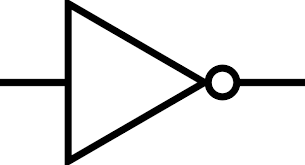
\includegraphics[scale=0.7]{notGate}
\end{center}
La porta logica \textit{NOT} ha in ingresso un segnale e manda in uscita il suo opposto.\\
Mappa quindi:
$0\rightarrow1$ e $1\rightarrow0$.
\section{Classiche (2 bit)}
\subsection{AND}
\begin{center}
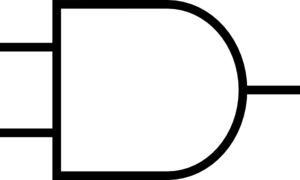
\includegraphics[scale=12]{andGate}
\end{center}
La porta logica \textit{AND} ha in ingresso due segnali e manda in uscita un segnale positivo se e solo se entrambi sono positivi.\\
Mappa quindi:\\
$\{1,1\}\rightarrow1$, $\{1,0\}\rightarrow0$, $\{0,1\}\rightarrow0,$ $\{0,0\}\rightarrow0$
\subsection{OR}
\begin{center}
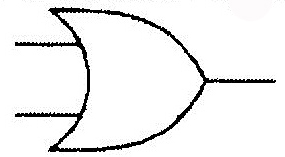
\includegraphics[scale=3]{orGate}
\end{center}
La porta logica \textit{OR} ha in ingresso due segnali e manda in uscita un segnale positivo se almeno uno è positivo.\\
Mappa quindi:\\
$\{1,1\}\rightarrow1$, $\{1,0\}\rightarrow1$, $\{0,1\}\rightarrow1,$ $\{0,0\}\rightarrow0$
\subsection{XOR}
\begin{center}
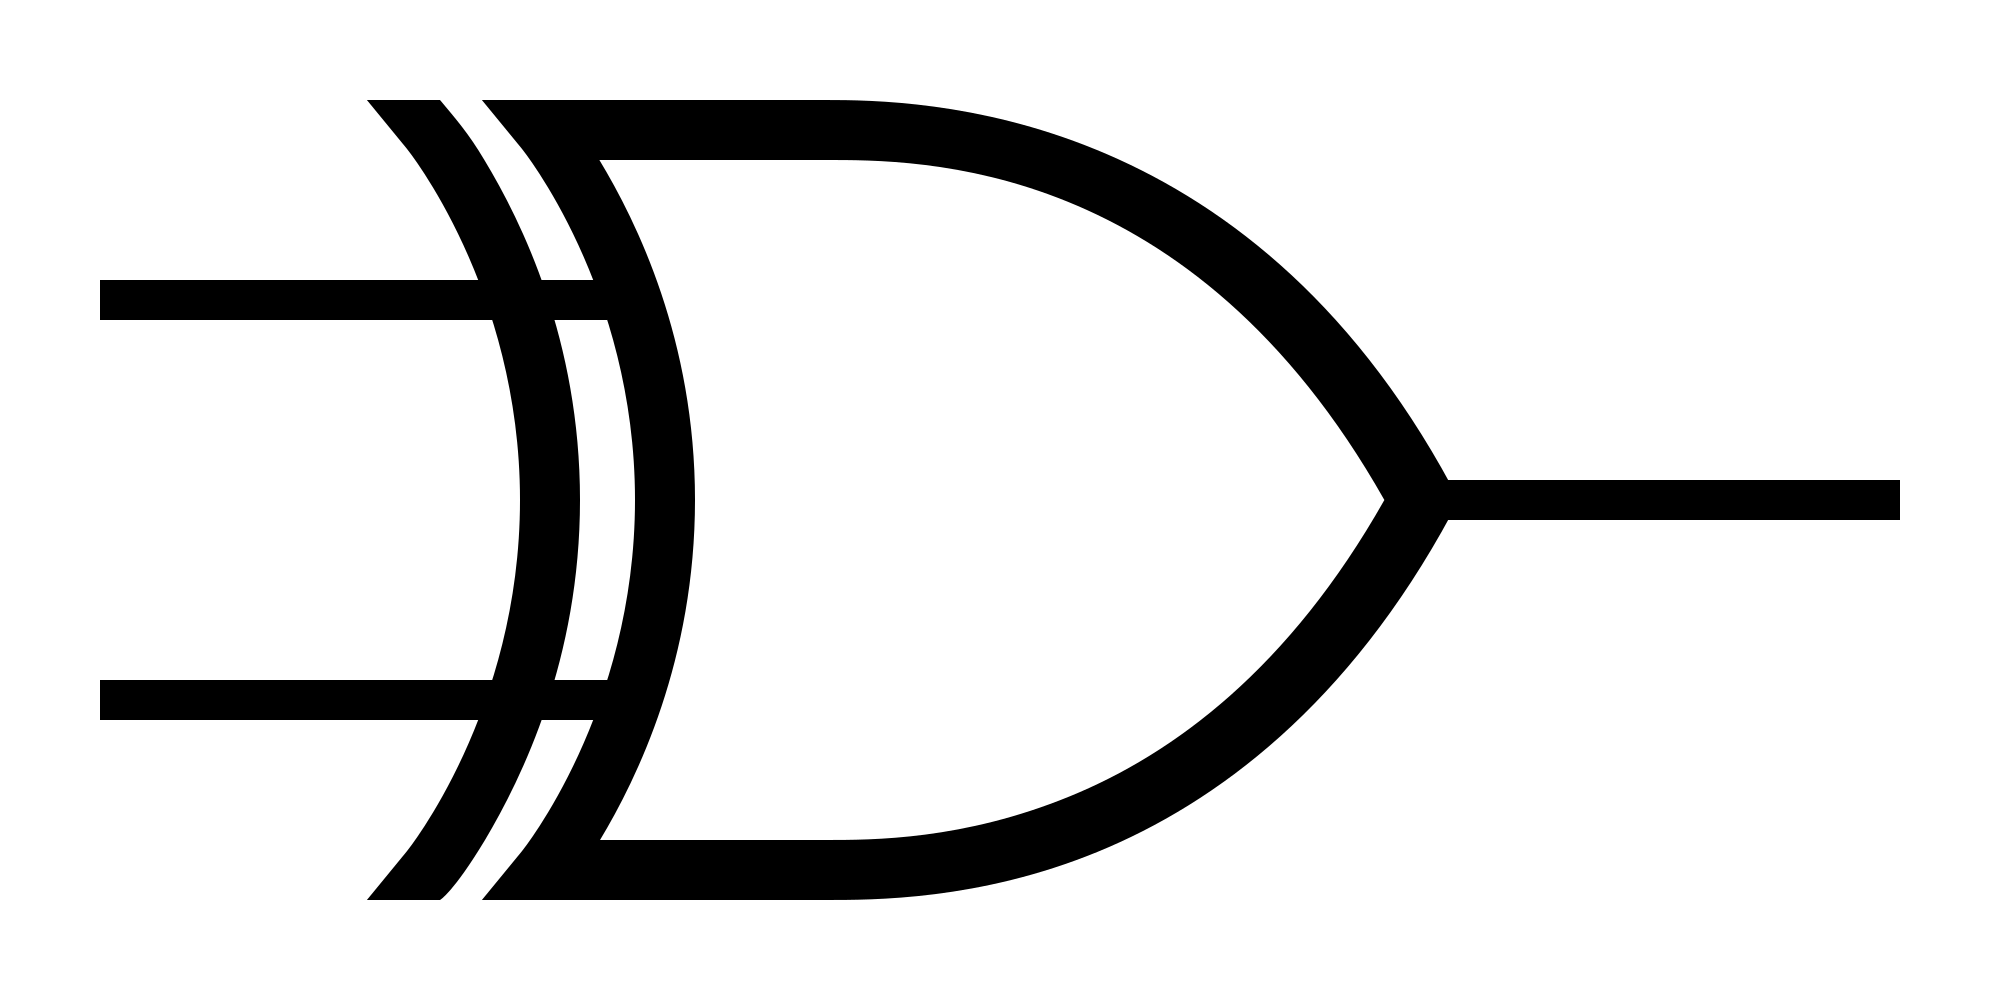
\includegraphics[scale=0.13]{xorGate}
\end{center}
La porta logica \textit{XOR} ha in ingresso due segnali e manda in uscita un segnale positivo se e solo se solo uno è positivo.\\
Mappa quindi:\\
$\{1,1\}\rightarrow0$, $\{1,0\}\rightarrow1$, $\{0,1\}\rightarrow1,$ $\{0,0\}\rightarrow0$
\subsection{Altre}
Esistono poi altre porte logiche, come la NAND o la NOR; ma non sono fondamentali in quanto ottenibili da una combinazione di quelle mostrate (ad esempio NAND = AND + NOT).\\
Porte logiche con più di due segnali di ingresso non vengono usate in quanto per computare più informazioni è sufficiente concatenare.
\section{Quantistiche (1 qubit)}
\subsection{Measurment}
Si tratta della misura di un qubit; non esattamente una porta logica, ma nel capitolo \textit{Cenni di meccanica quantistica} abbiamo visto che applica una trasformazione; misurando infatti il qubit collassa in autostato $\ket{0}$ oppure in $\ket{1}$ con una distribuzione di probabilità dipendente dallo stato del qubit. Per di più il valore viene salvato in un bit classico. Mappa quindi:\\
$\alpha\ket{0} + \beta\ket{1} \rightarrow \ket{0}$ con una probabilità di $|\alpha|^2$ oppure $\alpha\ket{0} + \beta\ket{1} \rightarrow \ket{1}$ con una probabilità di $|\beta|^2$
\subsection{X}
\begin{center}

\includegraphics[scale=1.25]{xGate}
\end{center}
La porta logica \textit{X} è conosciuta anche come \textit{bit-flip} in quanto inverte 0 con 1 e viceversa; è molto simile quindi alla porta classica \textit{NOT}. Mappa:\\
$\ket{1} \rightarrow \ket{0}$\\
$\ket{0} \rightarrow \ket{1}$\\
$\alpha\ket{0} + \beta\ket{1} \rightarrow \beta\ket{0} + \alpha\ket{1}$\\
La porta \textit{X} sulla BLOCH SPHERE applica una rotazione di $\pi$ radianti attorno all'asse x come si può vedere nell'immagine sottostante.
\begin{center}
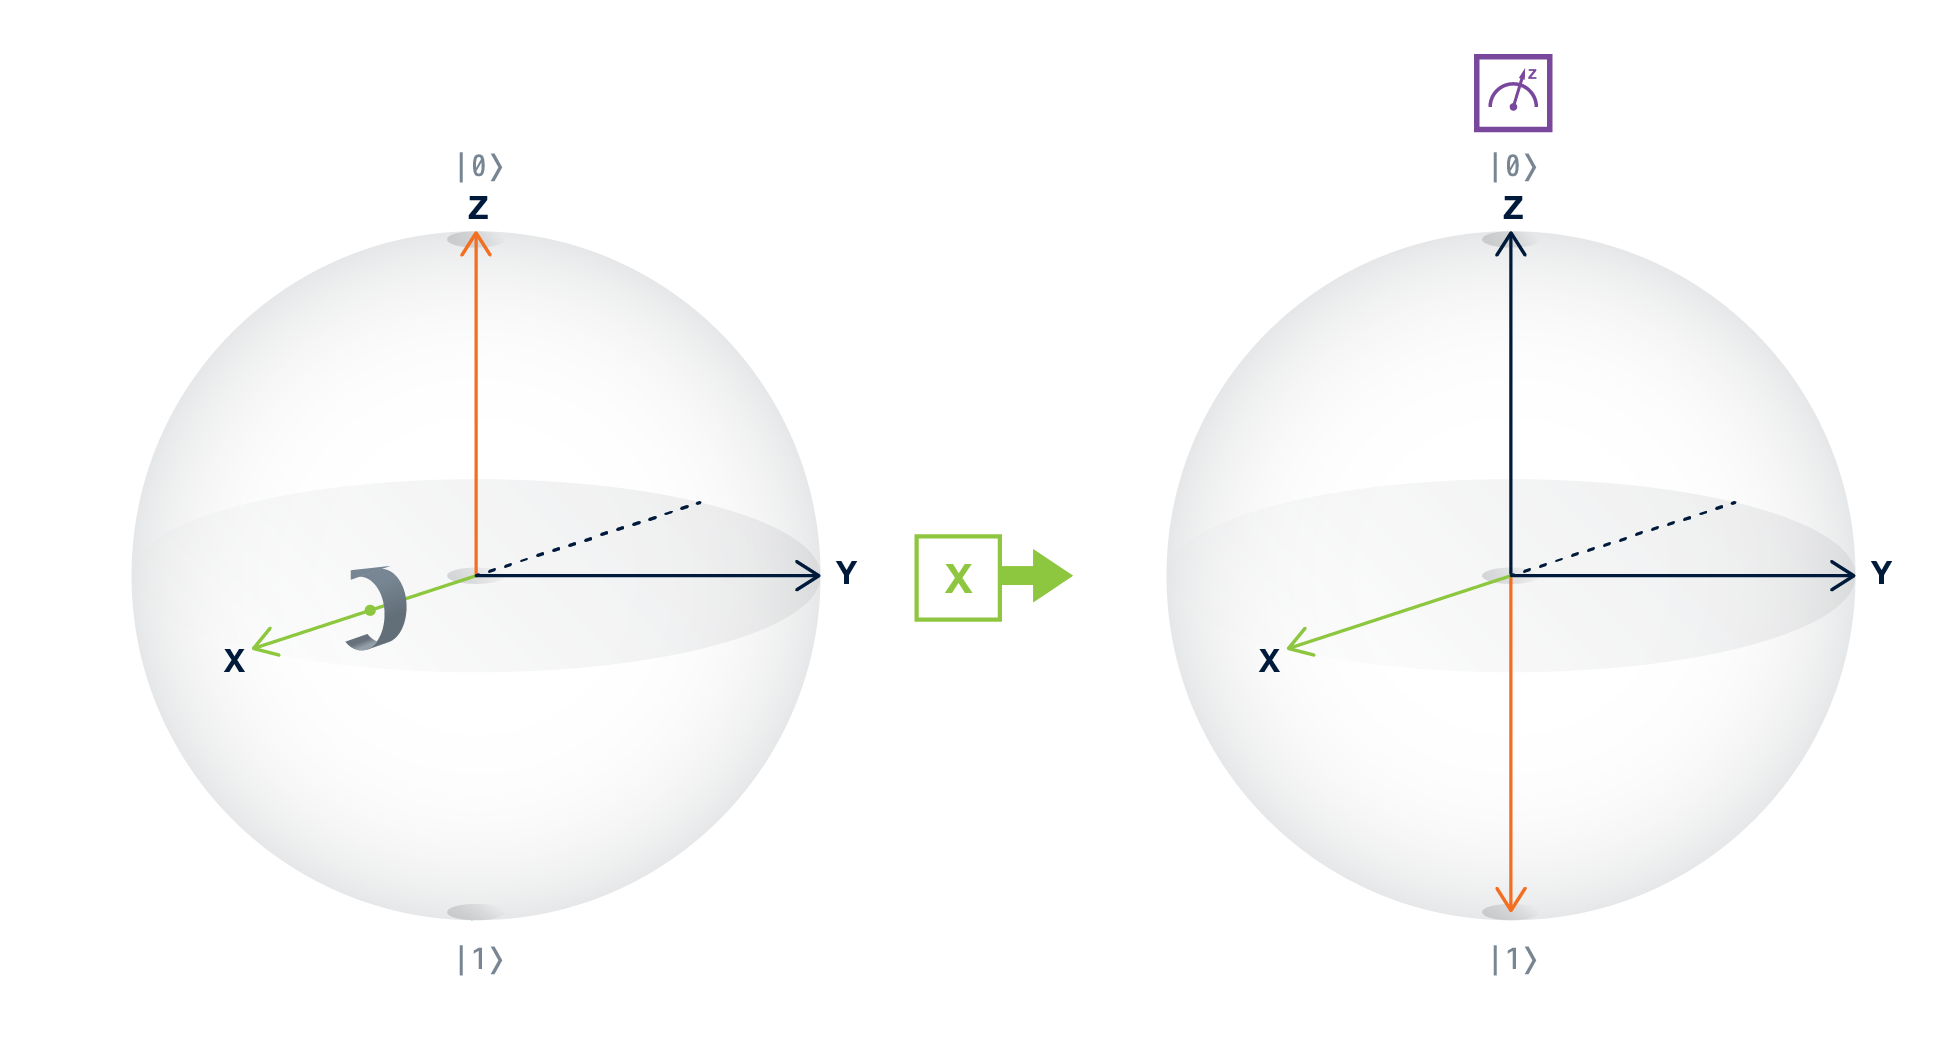
\includegraphics[scale=0.5]{xTrasformation}
\end{center}
\subsection{Hadamard}
\begin{center}

\includegraphics[scale=1]{hGate}
\end{center}
La porta di \textit{Hadamard} (o semplicemente \textit{H}) è forse la più importante delle macchine quantistiche in quanto permette al qubit di passare da un'autostato a una superposizione in cui 0 e 1 sono equiprobabili (non sarà ovviamente così se il qubit di partenza non è in un'autostato). Più precisamente si può osservare sulla BLOCH SPHERE che \textit{H} applica una rotazione di $\pi$ intorno agli assi X e Z.\\
Quello che accade agli autostati se applicato \textit{H}:\\
$\ket{0} \rightarrow \frac{1}{\sqrt{2}}(\ket{0} + \ket{1}) = \ket{+}$\\
$\ket{1} \rightarrow -\frac{1}{\sqrt{2}}(\ket{0} + \ket{1}) = \ket{-}$\\
$\ket{+}$ e $\ket{-}$ sono simboli rappresentanti i due vettori di stato che sulla BLOCH SPHERE puntano a +X e a -X. Da notare come $\frac{1}{\sqrt{2}}^2 = \frac{1}{\sqrt{2}}^2 = \frac{1}{2}$ e quindi in entrambi i casi 0 e 1 sono equiprobabili
\begin{center}
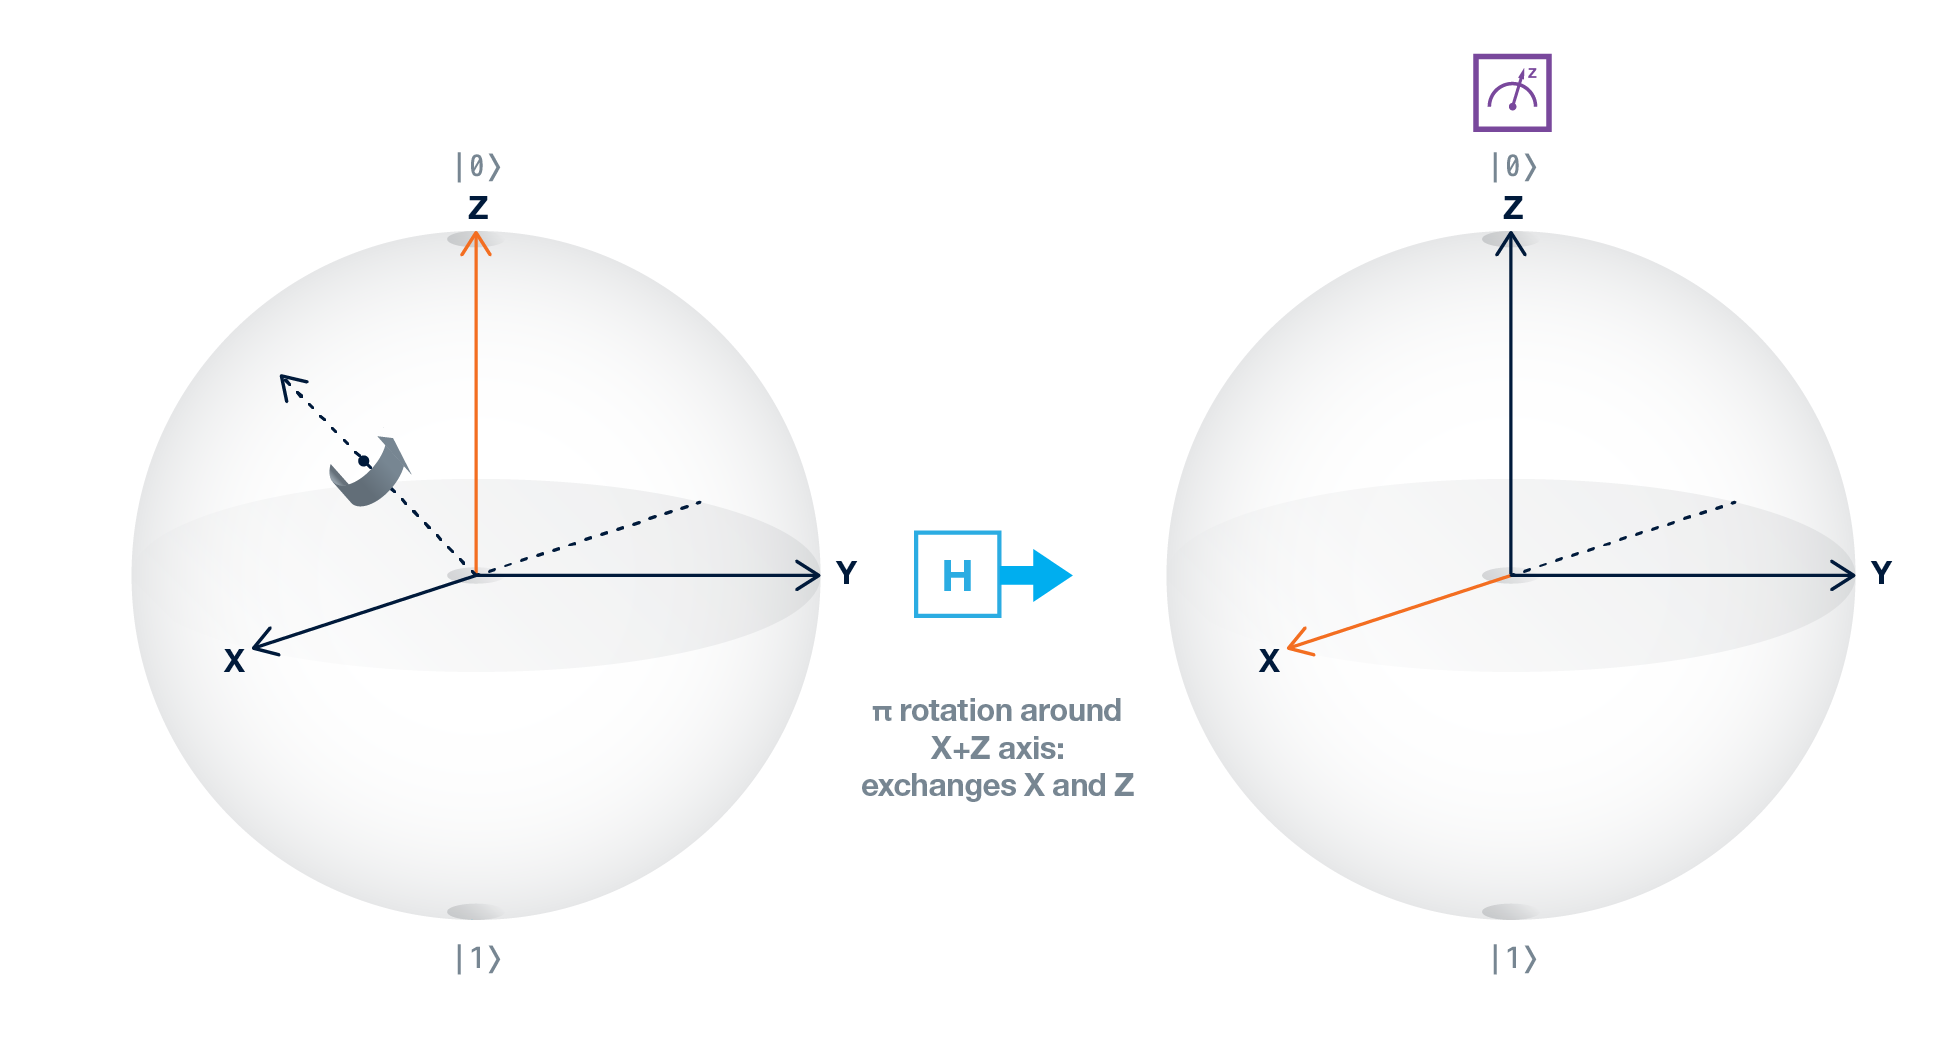
\includegraphics[scale=0.5]{hTrasformation}
\end{center}
\subsection{Z}
\begin{center}

\includegraphics[scale=0.77]{zGate}
\end{center}
La porta \textit{Z} porta ad una rotazione di $\pi$ intorno all'asse Z; gli autostati, essendo allineati, non vengono trasformati come si vede nell'immagine qui sotto.
\begin{center}
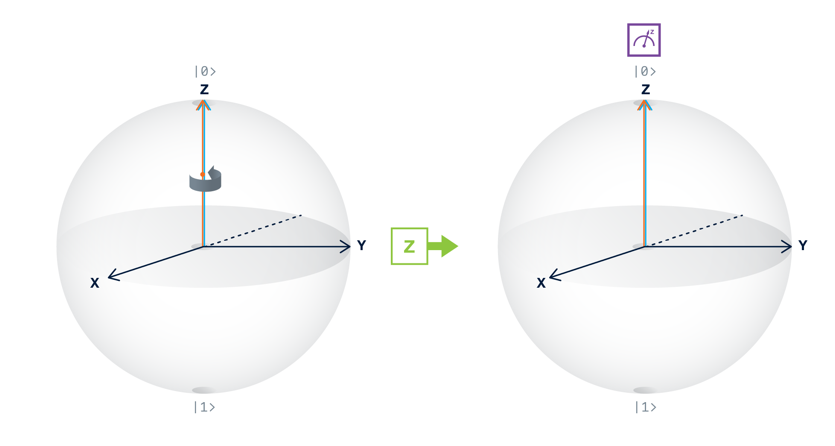
\includegraphics[scale=1.1]{zTrasformation}
\end{center}
Subiscono un effetto invece tutti gli altri vettori di stato, in particolare $\ket{+} \rightarrow \ket{-}$ e viceversa.
\begin{center}
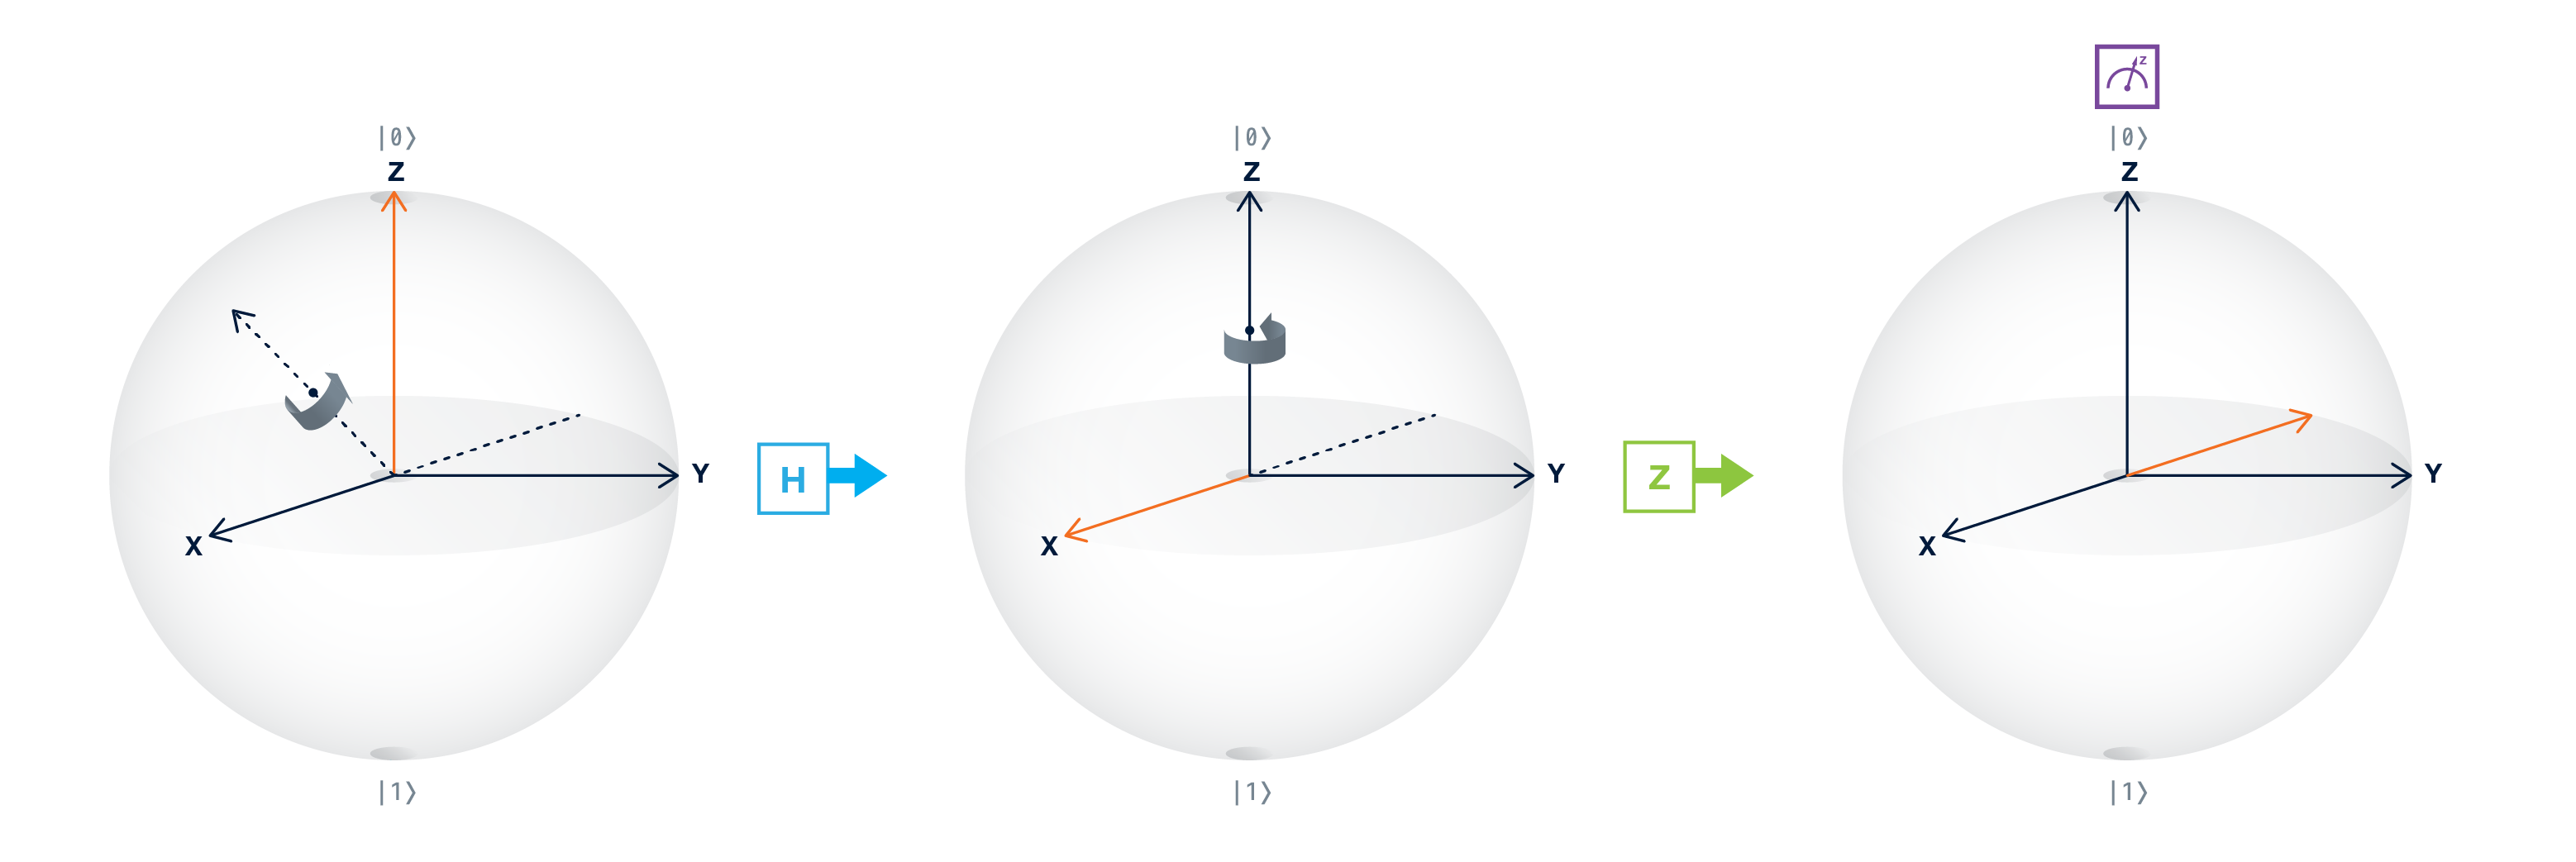
\includegraphics[scale=0.35]{hzTrasformation}
\end{center}
\subsection{S,T}
\begin{center}

\includegraphics[scale=0.77]{sGate}

\includegraphics[scale=0.77]{tGate}
\end{center}
I gate \textit{S} e \textit{T} sono molto simili a \textit{Z} solamente che applicano una rotazione rispettivamente di $\frac{\pi}{2}$ e $\frac{\pi}{4}$ intorno all'asse Z. Nell'immagine i vari esempi a partire da da $\ket{+}$
\begin{center}
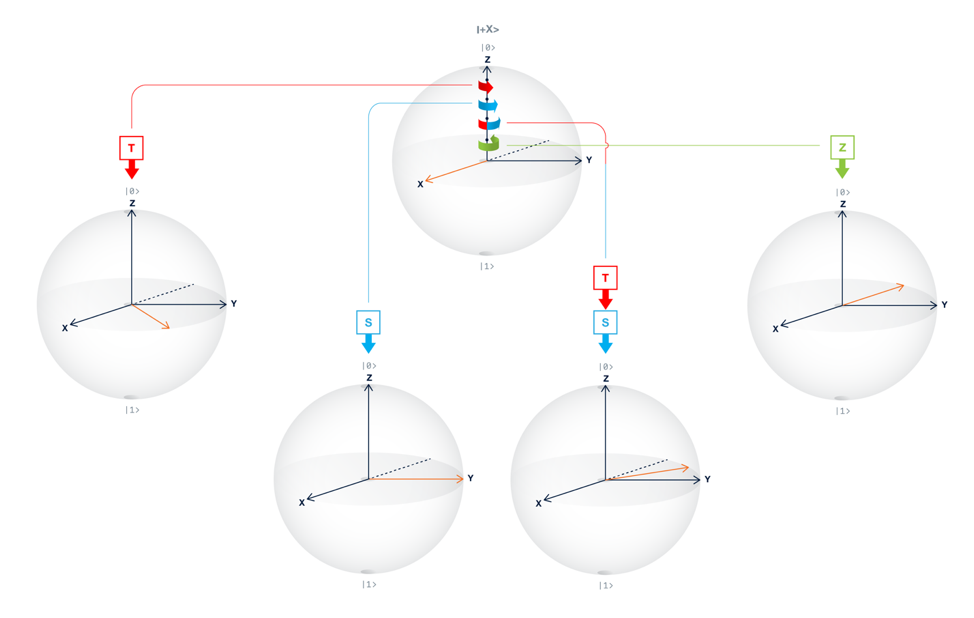
\includegraphics[scale=1.1]{stTrasformation}
\end{center}

\section{Quantistiche (2 qubit)}
\subsection{CNOT}
